

\section{Background} 
\label{sec:back}

There are several basic approaches to write an artificial intelligence (AI) for a game. In this project we were forced to investigate different ideas at three different research areas: heuristic based search, reinforcement learning and nature inspired algorithm. 
Of course there is an overlap between these approaches. All of them try to find the next best step for the agent by iterating through a search tree. This is build in base of all possible game steps that could done by the agent.
One naive approach of iterating through the whole search tree is not possible, because there is a time limitation.
Generally this leads to solve the trade-off between iterating similar to a breadth-first or depth-first search.
The heuristic approach forces the second by using a estimation function for looking many steps ahead.


\subsection{Heuristic Based Search} 

A heuristic is used to evaluate a game state by putting several facts into one number. When we have to decide which current active branch of a search tree should be iterated this score might help us. 
One common idea to estimate the distance to the target is the manhatten distance~\cite{distance_metrics}. 

In a two dimensional space the manhatten distance is calculated by

\begin{equation}
dist(u,v) = |x_{1} - x_{2}| + |y_{1} - y_{2}|
\end{equation}

adding the absolute value of the difference for the $x$ and the $y$ axis. The input consists always of the points that have one value for each dimension. This could be extended for a n-dimensional space as well. When thinking of a way at a grid this is always a path with one rectangle waypoint (see Figure ~\ref{fig:manhatten}).

\begin{figure}
\centering
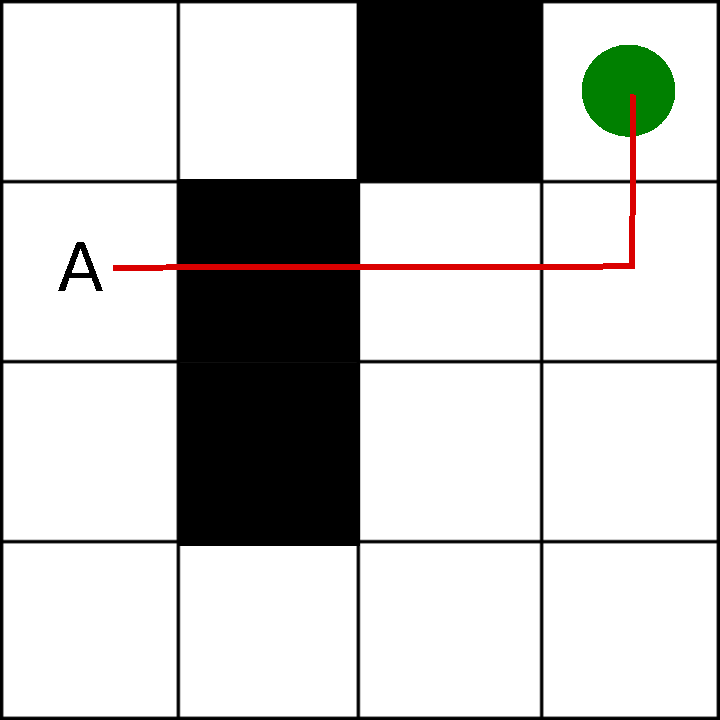
\includegraphics[scale=0.3]{images/manhatten.pdf}
\caption{Manhatten distance}
\label{fig:manhatten}
\end{figure}



\subsubsection{Greedy}

Greedy-algorithms are a whole class of algorithms and strategies. All of them follow a specific scheme/rule. They are iterative and choose in every step the state with the best reward. The state is in most cases a node which represents the state of the algorithm. The advantage of greedy algorithms is that they are very fast but on the other hand they are not optimal they often only find a local optima and not the global one. The advantage and disadvantage is caused by the greedy approach.  

\subsubsection{One Step Lookahead}

One step lookahead is a very simple tree search algorithm which follows the greedy approach. The actual state is the root node. From this node we only look one step ahead to all nodes which are connected by one edge and compute a heuristic value or another kind of reward value for these nodes. 

\begin{figure}
\centering
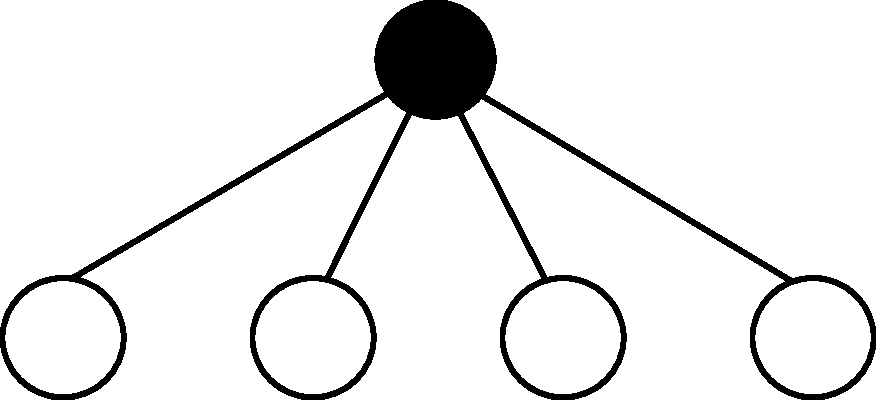
\includegraphics[scale=0.3]{images/onestep_lookahead.pdf}
\caption{Search tree for One Step Lookahead}
\label{fig:onestep}
\end{figure}


After that the algorithm terminates and we pick the node with the best value.

\subsubsection{AStar}

The A* tree search algorithm is a modification of the dijkstra algorithm and also belongs to the class of greedy algorithms. The Algorithm finds the shortest path between two nodes. In difference to normal greedy algorithms A* is a optimal algorithm, it finds a solution when a solution exists (in this case the shortest path). The algorithm uses a heuristic to estimate the shortest path. The value f(x) of a node N is the sum of its heuristic value h(x) and the costs from the start-node to N g(x).

\begin{equation}
f(x)=h(x)+g(x)
\end{equation}


A* contains two sets of nodes, the openlist and the closedlist. In every step of the algorithm the Node N with the lowest f(x) value in the openlist is put on the closedlist and all its connected nodes, which are not in the closedlist, are put in the openlist (with reference to their fahter N). If a connected node is already in the closedlist but the new generated value f'(x) is lower than f(x) then f(x) will be replaced by f'(x) and the new father-reference is N. The openlist contains all the nodes to which the path is already known and which can be checked in the next step, the closedlist contains every visited and checked node. When the actual node is the goal-node, the algorithm terminates. To generate the path, the algorithm goes back from the goal-node to the start node (guided by the father-references). 

\subsection{Reinforcement learning} 
 
Reinforcement learning, below RL, is a field in Machine learning which is a section of Artificial Intelligence. RL methods are mostly used by agents in an environment called Markov decision process, below MDP. MDP is a mathematical description of decision processes. They have different states S and some actions A which are available in the actual state. Every timestep the agent chooses an action $a$ and the process switches from state $s_a$ to $s_n$. The probability to go over form a state S to another state S' by any action A can be described as
\[
	G: S*S*A \rightarrow [0,1] 
\] 
and the reward given to the agent can be described by this:
\[
	R: S*S*A \rightarrow \mathbb{R}
\]
So that
\[
	(s_a, s_n, a) \rightarrow p(s_n|s_a, a)
\]
would describe the probability $p$ to go over in the state $s_n$, given the actual state $s_a$ and the choosen action $a$ and 
\[
	(s_a, s_n, a) \rightarrow r
\]
shows its corresponding reward.  


In differ to other learn methods and approaches like the (semi)supervised learning, RL algorithms never use information which they do not figured out themselves, so no correct samples were given to the algorithm. The only information is the reward given to the agent and some additional information like heuristic values, depending of the specific algorithm. 
A big problem problem in RL is the conflict between exploration of new and unvisited areas of the solution room and exploitation which is the improvement of already found solutions.
...
\subsubsection{Monte Carlo Tree Search} 

Monte Carlo Tree Search, below MCTS, is a class of RL algorithms. It is the most important concept in this paper. MCTS needs a tree of nodes which represent the different states, the edges represent the actions used by the agent to get to this node. The MCTS algorithm traverses to this tree and expands it. To find the global optimum a good balancing ratio between exploration and exploitation is required. 

[maybe picture from his paper and pseudocode]

The general MCTS algorithm has four steps, selection, expansion, simulation and backpropagation. In the selection the algorithm starts at  
freddy working on it 


\subsection{Nature inspired} 
The nature is solving problems by applying different approaches instinctively. 

\subsubsection{Neural nets} 
Our brain solves many problems that could not be solved by algorithms yet. Many researcher tries to explore the process of the human brain. Neural networks tries to model the nervous system and to adapt all the processes~\cite{nn_intro}. The neurons are modeled as \textit{threshold logic units} (TLU) that consists of several input values $x_1$ to $x_n$ and one output value $y$~\cite{ci_kruse}. 


\begin{figure}
\centering
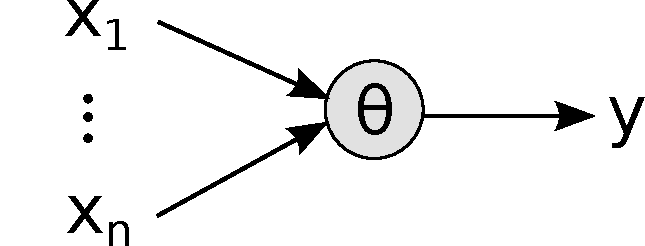
\includegraphics[scale=0.3]{images/tlu.pdf}
\caption{threshold logic units ~\cite{ci_kruse}}
\label{fig:tlu}
\end{figure}


For computing the output value is always for every input value one weight $w_i$ and the threshold $\theta$. The formula 

\begin{equation}
    y = 
\begin{dcases}
    1, & \text{if } \sum_{i=1}^n w_{i} x_{i} \geq \theta \text{,} \\
    0, & \text{otherwise.}
\end{dcases}
\end{equation}

is used to calculate the output $y$ that is either 0 or 1.
Normally the input and the output is given and the weights has to be learned. With only one TLU there only linear separable spaces could be learned perfectly.
To solve that problem there is the possibility to create a network of TLU's and map that problem to a higher dimensional space~\cite{ci_kruse}.




\subsubsection{Evolutionary algorithm} 
An \textit{Evolutionary Algorithm} (EA) tries to use the biological behavior of the population~\cite{evo}. 


\begin{algorithm}
\caption{Evolutionary Algorithm~\cite{evo}}
\label{alg:evo}
\begin{algorithmic}
\State \emph{Initialize} Population with random candidate solutions;
\State \emph{Evaluate} each candidate;
\While{Termination condition not satisfied} 
\State \emph{Select} parents;
\State \emph{Recombine} pairs of parents;
\State \emph{Mutate} the resulting offspring;
\State \emph{Evaluate} new candidates;
\State \emph{Select} individuals for the next generation;
\EndWhile
\end{algorithmic}
\end{algorithm}




\subsubsection{Pheromones} 



